\documentclass[nonacm,sigconf,fleqn,svgnames,screen]{acmart}
%%%%%%%%% DO NOT ALTER THIS, OPTIONAL PART STARTS BELOW %%%%%%%%%%%%

%%% Disable some standard ACM things that we don't want to see
\AtBeginDocument{%
  \providecommand\BibTeX{{%
    \normalfont B\kern-0.5em{\scshape i\kern-0.25em b}\kern-0.8em\TeX}}}

\setcopyright{none}
\copyrightyear{none}
\acmYear{none}
\acmDOI{none}


%%% ML2R colors
\definecolor{ml2rblu}{rgb}{0.02,0.27,0.45}
\definecolor{ml2ryel}{rgb}{0.98,0.72,0.18}
\definecolor{ml2rgrn}{rgb}{0.50,0.71,0.18}
\definecolor{ml2rtrq}{rgb}{0.00,0.57,0.57}

%%% not yet imported by ACM style
% \usepackage{amssymb}
\usepackage{amsthm}
\usepackage{mathtools}
\usepackage{bm}
\usepackage[font=footnotesize]{subfig}
\usepackage{booktabs}
\usepackage{array}
\usepackage{fixltx2e}
\usepackage{nicefrac}

\usepackage{wasysym}

\usepackage{tikz}
\usetikzlibrary{shapes.geometric, positioning}

\usepackage{algorithm}
\usepackage[noend]{algpseudocode}
\renewcommand{\algorithmiccomment}[1]{{\color{DarkRed!90}// #1}}

\usepackage{hyperref}
\hypersetup{%
  colorlinks=true,
  urlcolor=ml2rtrq,
  linkcolor=ml2rtrq,
  citecolor=ml2rtrq,
  bookmarks=false}


\usepackage{fancyvrb} 
\usepackage{listings}
% Python style / environment for highlighting in "figures"
\lstdefinestyle{pythonstyle}{%
  language=Python,
  tabsize=4,
  backgroundcolor=\color{Gray!10},
  basicstyle=\ttfamily\scriptsize,
  stringstyle=\color{ForestGreen},
  keywordstyle=\color{BlueViolet},
  commentstyle=\itshape\color{DarkRed!90},
  identifierstyle=,
  emphstyle=\color{Blue},
  frame=lines,	
  showstringspaces=false,
  morekeywords={range, len, self, other, lambda, from, import, as, False, True, 
  enumerate, xrange, map, list, set, float, int, min, max, sorted, None},
  fancyvrb=true,
}
\lstnewenvironment{python}[1][]{\lstset{style=pythonstyle,#1}}{}

% Python style / environment for highlighting in body
\lstdefinestyle{pythonstyletxt}{%
  language=Python,
  tabsize=4,
  basicstyle=\ttfamily\small,
  stringstyle=\color{ForestGreen},
  keywordstyle=\color{BlueViolet},
  commentstyle=\itshape\color{DarkRed!90},
  identifierstyle=,
  emphstyle=\color{Blue},
  %frame=l,	
  xleftmargin=1em,
  showstringspaces=false,
  morekeywords={range, len, self, other, lambda, from, import, as, False, True, 
  enumerate, xrange, map, list, set, float, int, min, max, sorted, with, None},
}
\lstnewenvironment{pythontxt}[1][]{\lstset{style=pythonstyletxt,#1}}{}

% Python style / environment for small size highlighting in body
\lstdefinestyle{pythonstyletxtsmall}{%
  language=Python,
  tabsize=4,
  basicstyle=\ttfamily\scriptsize,
  stringstyle=\color{ForestGreen},
  keywordstyle=\color{BlueViolet},
  commentstyle=\itshape\color{DarkRed!90},
  identifierstyle=,
  emphstyle=\color{Blue},
  %frame=l,	
  xleftmargin=1em,
  showstringspaces=false,
  morekeywords={range, len, self, other, lambda, from, import, as, False, True, 
  enumerate, xrange, map, list, set, float, int, min, max, sorted, None},
}
\lstnewenvironment{pythontxtsmall}[1][]{\lstset{style=pythonstyletxtsmall,#1}}{}


\newcommand{\putORCID}[1]{
\authornote{\href{https://orcid.org/#1}{
\includegraphics[width=2ex]{ORCID.png}} \href{https://orcid.org/#1}{#1}}
\orcid{#1}}



%%%%%%%% OPTIONAL %%%%%%%%%%%%%%%

% only used for fig colors, may be removed if you don't need it
\usepackage{tikz}
\usetikzlibrary{shapes.geometric, positioning}

%%% define convience commands
% python stuff
\newcommand{\Py}{\emph{Python}}
\newcommand{\PY}{\emph{Python }}
\newcommand{\NP}{\emph{NumPy }}
\newcommand{\Np}{\emph{NumPy}}
\newcommand{\SP}{\emph{SciPy }}
\newcommand{\Sp}{\emph{SciPy}}
\newcommand{\MP}{\emph{Matplotlib }}
\newcommand{\Mp}{\emph{Matplotlib}}
\newcommand{\NX}{\emph{NetworkX }}
\newcommand{\Nx}{\emph{NetworkX}}
\newcommand{\QT}{\emph{QuTiP }}
\newcommand{\Qt}{\emph{QuTiP}}

% text highlighting
\newcommand{\alert}[1]{\emph{#1}}
\newcommand{\ALERT}[1]{{\color{red}#1}}
\newcommand{\keyword}[1]{\emph{\texttt{\color{blue}#1}}}

% vectors, matrices, and tensors
\renewcommand{\vec}[1]{\bm{#1}}
\newcommand{\mat}[1]{\bm{#1}}
\newcommand{\ten}[1]{\bm{\mathcal{#1}}}

% transposition
\newcommand{\trn}[1]{#1^\intercal}

%%% inner, outer products and squared Euclidean norms/distances
\newcommand{\IPA}[2]{\Bigl \langle #1 \bigm| #2 \Bigr \rangle}
\newcommand{\Ipa}[2]{\bigl \langle #1 \bigm| #2 \bigr \rangle}
\newcommand{\ipa}[2]{\left \langle #1 \,\middle|\, #2 \right \rangle}
%\newcommand{\ipt}[2]{#1^{\scriptscriptstyle T} #2}
\newcommand{\ipt}[2]{\trn{#1} #2}
%\newcommand{\ipt}[2]{#1^\intercal #2}
%\newcommand{\ipt}[2]{#1^\top #2}
%\newcommand{\ipt}[2]{#1^\mathsf{T} #2}
\newcommand{\opt}[2]{#1 \trn{#2}}
\newcommand{\nrm}[1]{\bigl \lVert #1 \bigr \rVert^2}
\newcommand{\NRM}[1]{\Bigl \lVert #1 \Bigr \rVert^2}
\newcommand{\dsq}[2]{\bigl \lVert #1 - #2 \bigr \rVert^2}
\newcommand{\DSQ}[2]{\Bigl \lVert #1 - #2 \Bigr \rVert^2}
\newcommand{\dist}[2]{\bigl \lVert #1 - #2 \bigr \rVert}
\DeclareMathOperator*{\vbar}{\Bigr\rvert}

%%% inner and outer product for indexed vectors
\newcommand{\iipt}[2]{\trn{#1} #2^{\phantom{\intercal}}}
\newcommand{\oipt}[2]{#1^{\phantom{\intercal}} \trn{#2}}

%%% trace and rank operator
\newcommand{\tr}[1]{\operatorname{tr} \bigl [ #1 \bigr ]}
\newcommand{\TR}[1]{\operatorname{tr} \Bigl [ #1 \Bigr ]}
\newcommand{\rk}[1]{\operatorname{rk} \bigl [ #1 \bigr ]}
\newcommand{\RK}[1]{\operatorname{rk} \Bigl [ #1 \Bigr ]}
\newcommand{\diag}[1]{\operatorname{diag} \bigl [ #1 \bigr ]}
\newcommand{\DIAG}[1]{\operatorname{diag} \Bigl [ #1 \Bigr ]}

%%% sets and optimization routines
\newcommand{\set}[1]{\mathcal{#1}}
\newcommand{\st}{\operatorname{s.\!t.}}
\newcommand{\amin}[1]{\operatorname*{argmin}_{#1}}
\newcommand{\amax}[1]{\operatorname*{argmax}_{#1}}

\newcommand{\submax}[1]{#1_{\max}}

%%% conditional independence and probability
\newcommand{\ci}{\perp\!\!\!\perp}
\newcommand{\prob}[1]{p\bigl( #1 \bigr)}
\newcommand{\cprob}[2]{p\bigl( #1 \mid #2 \bigr)}

%%% bras and kets
\newcommand{\ket}[1]{\vert {#1} \rangle}
\newcommand{\Ket}[1]{\big\vert {#1} \big\rangle}
\newcommand{\bra}[1]{\langle {#1} \vert}
\newcommand{\Bra}[1]{\big\langle {#1} \big\vert}
\newcommand{\braket}[2]{\langle {#1} \vert {#2} \rangle}
\newcommand{\Braket}[2]{\big\langle {#1} \big\vert {#2} \big\rangle}
\newcommand{\ketbra}[2]{\vert {#1} \rangle \langle {#2} \vert}
\newcommand{\Ketbra}[2]{\big\vert {#1} \big\rangle \big\langle {#2} \big\vert}

\newcommand{\hdash}{\operatorname{\,{}---{}\,}}
\renewcommand{\vdash}{\arrowvert}




\begin{document}

% set up pdf meta data
\hypersetup{%
  pdftitle={ML2R Coding Nuggets: Linear Programming},
  pdfauthor={Pascal Welke and Christian Bauckhage},
  pdfsubject={data science, machine learning, optimization, scientific python, numpy, scipy},
  pdfkeywords={linear programming, robust regression, least absolute deviations}
}


\title[Linear Programming for Robust Regression]{ML2R Coding Nuggets \\ Linear Programming for Robust Regression}


% This is how you define multiple authors
\author[P. Welke]{Pascal Welke}
\putORCID{0000-0002-2123-3781}
\affiliation{
  \institution{Machine Learning Rhine-Ruhr \\ University of Bonn}
  \city{Bonn}
  \state{Germany}
}

\author[C. Bauckhage]{Christian Bauckhage}
\putORCID{0000-0001-6615-2128}
\affiliation{
  \institution{Machine Learning Rhine-Ruhr \\ Fraunhofer IAIS}
  \city{St.~Augustin}
  \state{Germany}
}

\begin{abstract}
The ML2R Coding Nugget template defines a common look and feel for ML2R coding nuggets. 
The source code of this document shows how to use the ML2R Coding Nugget Template to produce nice documents.
\end{abstract}

\maketitle



\section{Introduction}
Coding nuggets are currently (short) how-tos that show how to solve problems ``by foot'' in practice.
The typical structure of such a paper consists of motivating a (machine learning) problem, showing how to formulate this problem in a particular way and then showing how to solve it practically using existing methods. 

Examples include  ``Solving Linear Programming Problems'' \cite{Welke2020-SLP} and ``Linear Programming for Robust Regression'' \cite{Welke2020-SLP2}.
In the latter example, e.g. we show how to fit a linear model to data by minimizing least absolute deviations, instead of the more common least squares. 
To this end, we formulate the optimization problem, transform it to show that it can be solved by linear programming and then solve it in \keyword{python} using methods from \keyword{numpy} and \keyword{scipy} alone.  

\section{Technical Details}
\verb+preamble.tex+ contains several imports and definitions. 
There is a part marked optional that you can change, remove or add to as you please. 
Please refrain from changing the part, however, that is marked as non-optional.
Below we give a short introduction to 

\subsection{Colors}
The preamble defines the ML2R corporate design colors that should be used throughout the document and within figures (cf. Fig.~\ref{colors}) to provide a common look and feel:

\vspace{0.5em}
\begin{center}
\begin{tabular}{lcl}
\textcolor{ml2rblu}{blue} & : & \textcolor{ml2rblu}{ml2rblu} \\
\textcolor{ml2ryel}{yellow} & : & \textcolor{ml2ryel}{ml2ryel} \\
\textcolor{ml2rgrn}{green} & : & \textcolor{ml2rgrn}{ml2rgrn} \\
\textcolor{ml2rtrq}{turquoise} & : & \textcolor{ml2rtrq}{ml2rtrq} \\
 \end{tabular} 
\end{center}

\begin{figure}
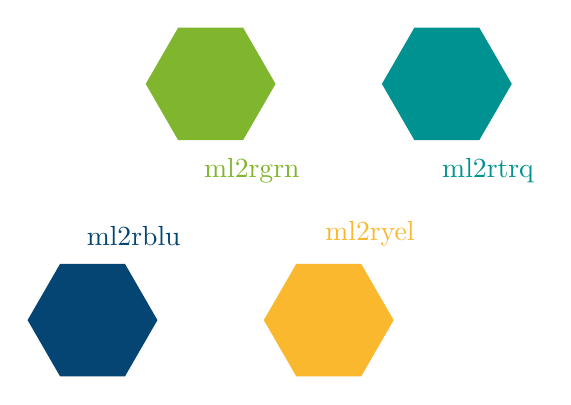
\begin{tikzpicture}
\node[regular polygon, regular polygon sides=6, draw,
inner sep=0.5cm, draw=ml2rblu, fill=ml2rblu] (blu) at (0,0) {};
\node[regular polygon, regular polygon sides=6, draw,
inner sep=0.5cm, draw=ml2ryel, fill=ml2ryel] (yel) at (3,0) {};
\node[regular polygon, regular polygon sides=6, draw,
inner sep=0.5cm, draw=ml2rgrn, fill=ml2rgrn] (grn) at (1.5,3) {};
\node[regular polygon, regular polygon sides=6, draw,
inner sep=0.5cm, draw=ml2rtrq, fill=ml2rtrq] (trq) at (4.5,3) {};
\node[above=3mm of blu.north east] {\textcolor{ml2rblu}{ml2rblu}};
\node[above=3mm of yel.north east] {\textcolor{ml2ryel}{ml2ryel}};
\node[below=3mm of grn.south east] {\textcolor{ml2rgrn}{ml2rgrn}};
\node[below=3mm of trq.south east] {\textcolor{ml2rtrq}{ml2rtrq}};
\end{tikzpicture}
\caption{A figure with our corporate design colors}
\label{colors}
\end{figure}

\subsection{Python Code and keywords}

Python code with pretty printing is supported. 
Inline code looks like this:
\begin{pythontxt}
vecWLAD = result.x[:m]
print('w0 =',vecWLAD[0])
print('w1 =',vecWLAD[1])
\end{pythontxt}

An example of a longer, floating python code environment can be found in Listing~\ref{code}.


\begin{python}[float=t!, caption={setting up a linear programming problem}, label={code}, emph={}, numbers=left, numbersep=5pt]
matA = np.zeros((2*n, m+n))
matA[:n,:m] = +matF.T
matA[n:,:m] = -matF.T
matA[:n,m:] = -np.eye(n)
matA[n:,m:] = -np.eye(n)

vecB = np.zeros(2*n)
vecB[:n] = +vecY
vecB[n:] = -vecY

vecC = np.hstack((np.zeros(m), np.ones(n)))
\end{python}


\section*{Acknowledgments} % should always be present. You may change the letter in the grant no. according to your institution(s)

This material was produced within the Competence Center for Machine Learning Rhine-Ruhr (\href{https://www.ml2r.de}{\bf ML2R}) which is funded by the Federal Ministry of Education and Research of Germany (grant no. 01|S18038C). The authors gratefully acknowledge this support.


\bibliographystyle{ACM-Reference-Format}
\bibliography{literature}


\end{document}
